\documentclass[11  pt]{exam} 
\usepackage[lmargin=1in,rmargin=1.75in,bmargin=1in,tmargin=.5in]{geometry}  


% For hyperlinking everything
\usepackage{hyperref}
\hypersetup{
	colorlinks=true, %set true if you want colored links
	linktoc=all,     %set to all if you want both sections and subsections linked
	linkcolor=blue,  %choose some color if you want links to stand out
}


\usepackage[latin1]{inputenc}
\usepackage{amsmath}
\usepackage{mathrsfs}  
\usepackage{amsfonts}
\usepackage{amssymb}
\usepackage{graphicx}
\usepackage{subfig}
\usepackage{caption}
\usepackage{algorithm}
%\usepackage{algcompatible}
%\usepackage{algorithmicx}
\usepackage{algpseudocode}

\usepackage{titlesec}
\titleformat{\section}{\fontfamily{lmss}\fontsize{14}{15}\bfseries}{\thesection}{1em}{}
\titleformat{\subsection}{\fontfamily{lmss}\fontsize{12}{15}\bfseries}{\thesubsection}{1em}{}




\usepackage{amsthm}

\newtheoremstyle{noit}
{10pt}% <Space above>
{10pt}% <Space below>
{}% <Body font>
{}% <Indent amount>
{\bfseries}% <Theorem head font>
{.}% <Punctuation after theorem head>
{.5em}% <Space after theorem headi>
{}% <Theorem head spec (can be left empty, meaning `normal')>

\newtheoremstyle{example}
{10pt}% <Space above>
{10pt}% <Space below>
{}% <Body font>
{20pt}% <Indent amount>
{\bfseries}% <Theorem head font>
{.}% <Punctuation after theorem head>
{.5em}% <Space after theorem headi>
{}% <Theorem head spec (can be left empty, meaning `normal')>


\newtheoremstyle{indented}{20pt}{20pt}{\addtolength{\leftskip}{2.5em}}{}{\bfseries}{.}{.5em}{}


\newtheorem{theorem}{Theorem}
\numberwithin{theorem}{section}
\newtheorem{lemma}[theorem]{Lemma}
\newtheorem{corollary}[theorem]{Corollary}
\newtheorem{observation}{Observation}
%\numberwithin{observation}{section}
%\numberwithin{definition}{section}
\newtheorem{conjecture}{Conjecture}
\newtheorem{Qu}{Question}
\newcommand{\QU}{\begin{Qu}\normalfont}

\theoremstyle{noit}
\newtheorem{fact}{Fact}
\newtheorem{definition}{Definition}

\theoremstyle{indented}
\newtheorem{example}{Example}

\theoremstyle{indented}
\newtheorem{problem}{Problem}


%\newenvironment{proof}{\noindent{\bf Proof:} \hspace*{1em}}{
%    \hspace*{\fill} $\Box$ }
%\newenvironment{proof_of}[1]{\noindent {\bf Proof of #1:}
%    \hspace*{1em} }{\hspace*{\fill} $\Box$ }
%\newenvironment{proof_claim}{\begin{quotation} \noindent}{
%    \hspace*{\fill} $\diamond$ \end{quotation}}
\newcommand{\vs}[1]{\vspace{#1}}

\newcommand{\lecture}[2]{
 \noindent
\begin{center}
	\framebox{
		\vbox{
			\hbox to 5.78in { {\bf CSCE 411: Design and Analysis of Algorithms} \hfill  }
			\vspace{2mm}
			\hbox to 5.78in { {\Large \hfill Lecture #1\hfill} }
			\vspace{2mm}
			\hbox to 5.78in { {\it Date: #2 \hfill Lecturer: Nate Veldt} }
		}
	}
\end{center}
\vspace*{4mm}
}


\newcommand{\hw}[2]{
	\noindent
	\begin{center}
		\framebox{
			\vbox{
				\hbox to 5.78in { {\bf CSCE 411: Design and Analysis of Algorithms} \hfill  }
				\vspace{2mm}
				\hbox to 5.78in { {\Large \hfill Homework #1\hfill} }
				\vspace{2mm}
				\hbox to 5.78in { {\it Due date: #2 \hfil} }
			}
		}
	\end{center}
	\vspace*{4mm}
}



\newcommand{\under}[1]{\underline{\hspace{#1}}}
\setlength{\parindent}{0em}

%\usepackage[tagged]{accessibility}

% Graph terms
\newcommand{\vol}{\textbf{vol}}
\newcommand{\cut}{\textbf{cut}}


% Matrices
\newcommand{\mA}{\textbf{A}}
\newcommand{\mB}{\textbf{B}}

% vectors
\newcommand{\ve}{\textbf{e}}
\newcommand{\vx}{\textbf{x}}


% Other
\newcommand{\calN}{\mathcal{N}}

\usepackage{mathtools}
\DeclarePairedDelimiter\ceil{\lceil}{\rceil}
\DeclarePairedDelimiter\floor{\lfloor}{\rfloor}


\newcommand*{\aitem}{ \item[{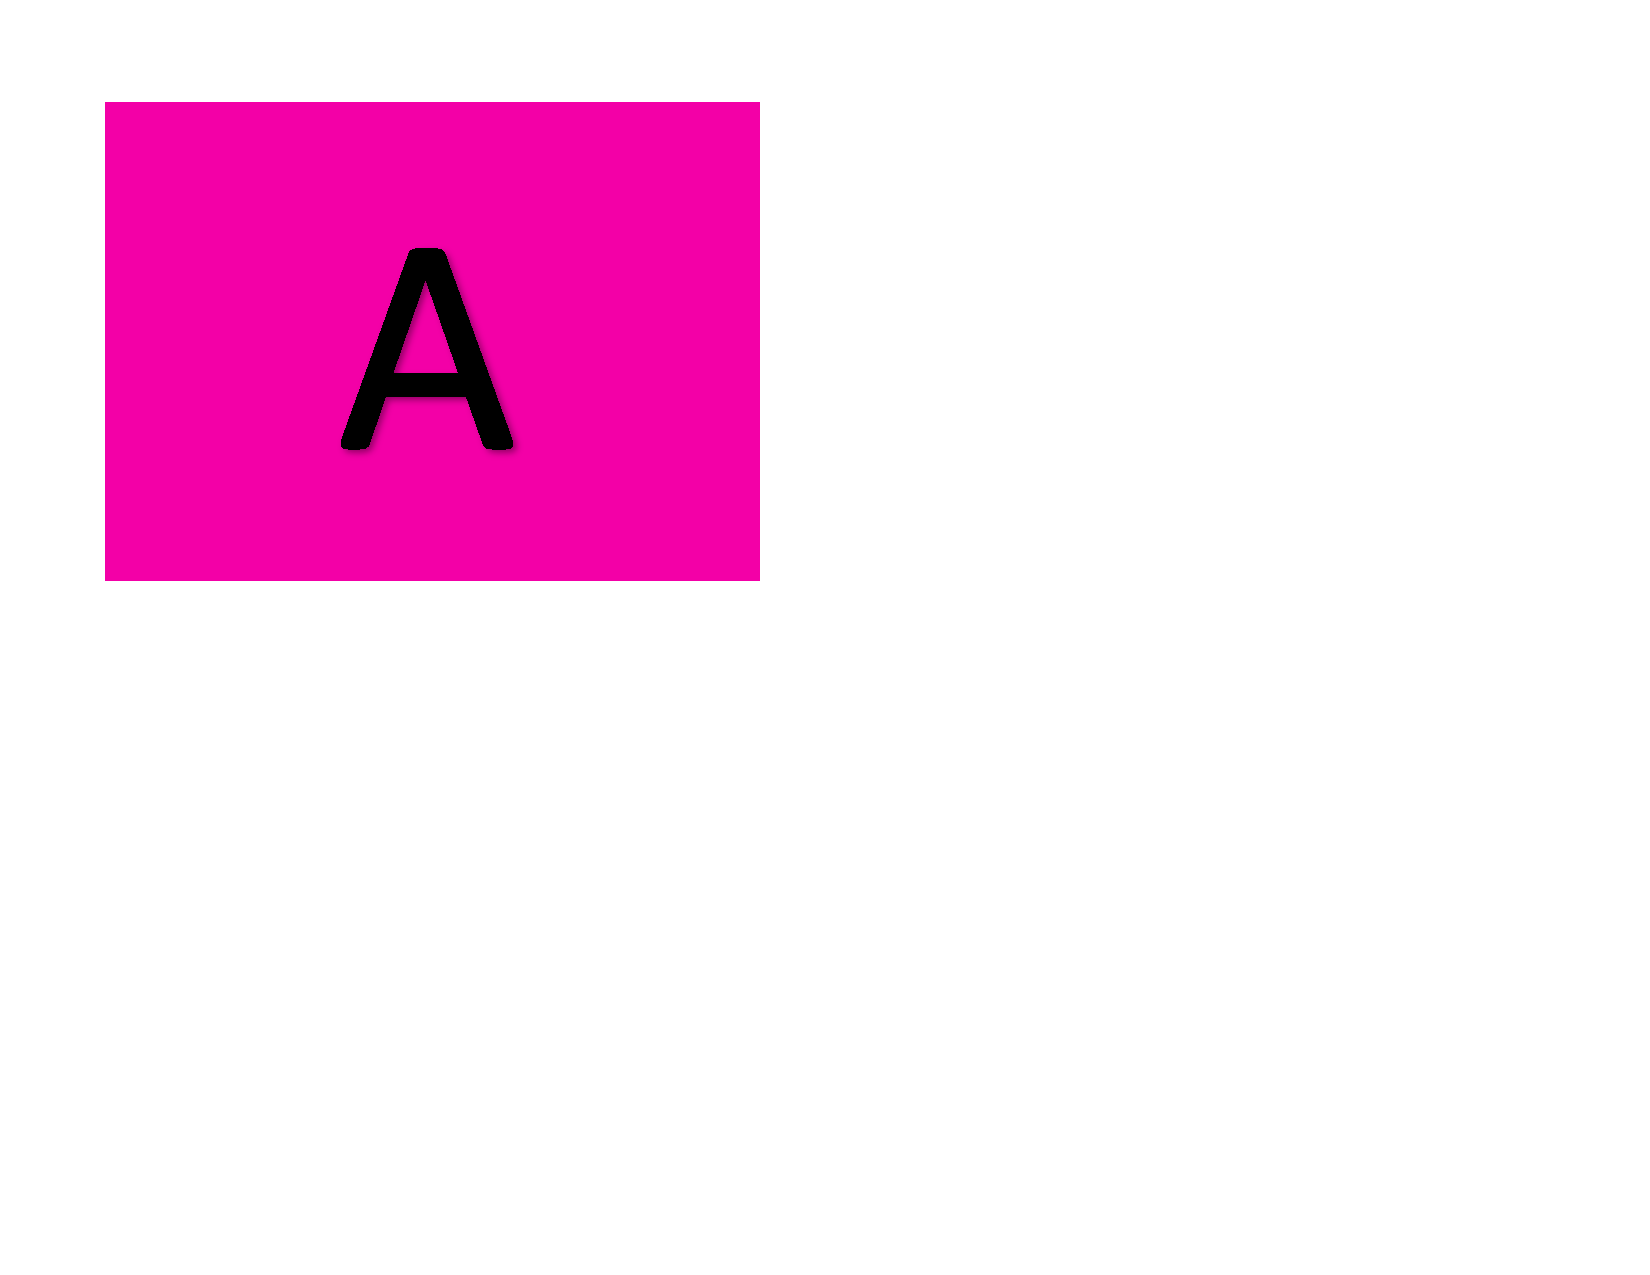
\includegraphics[width=0.8cm,height=0.5cm]{../../Lectures/figures/A}} ]  }
\newcommand*{\bitem}{ \item[{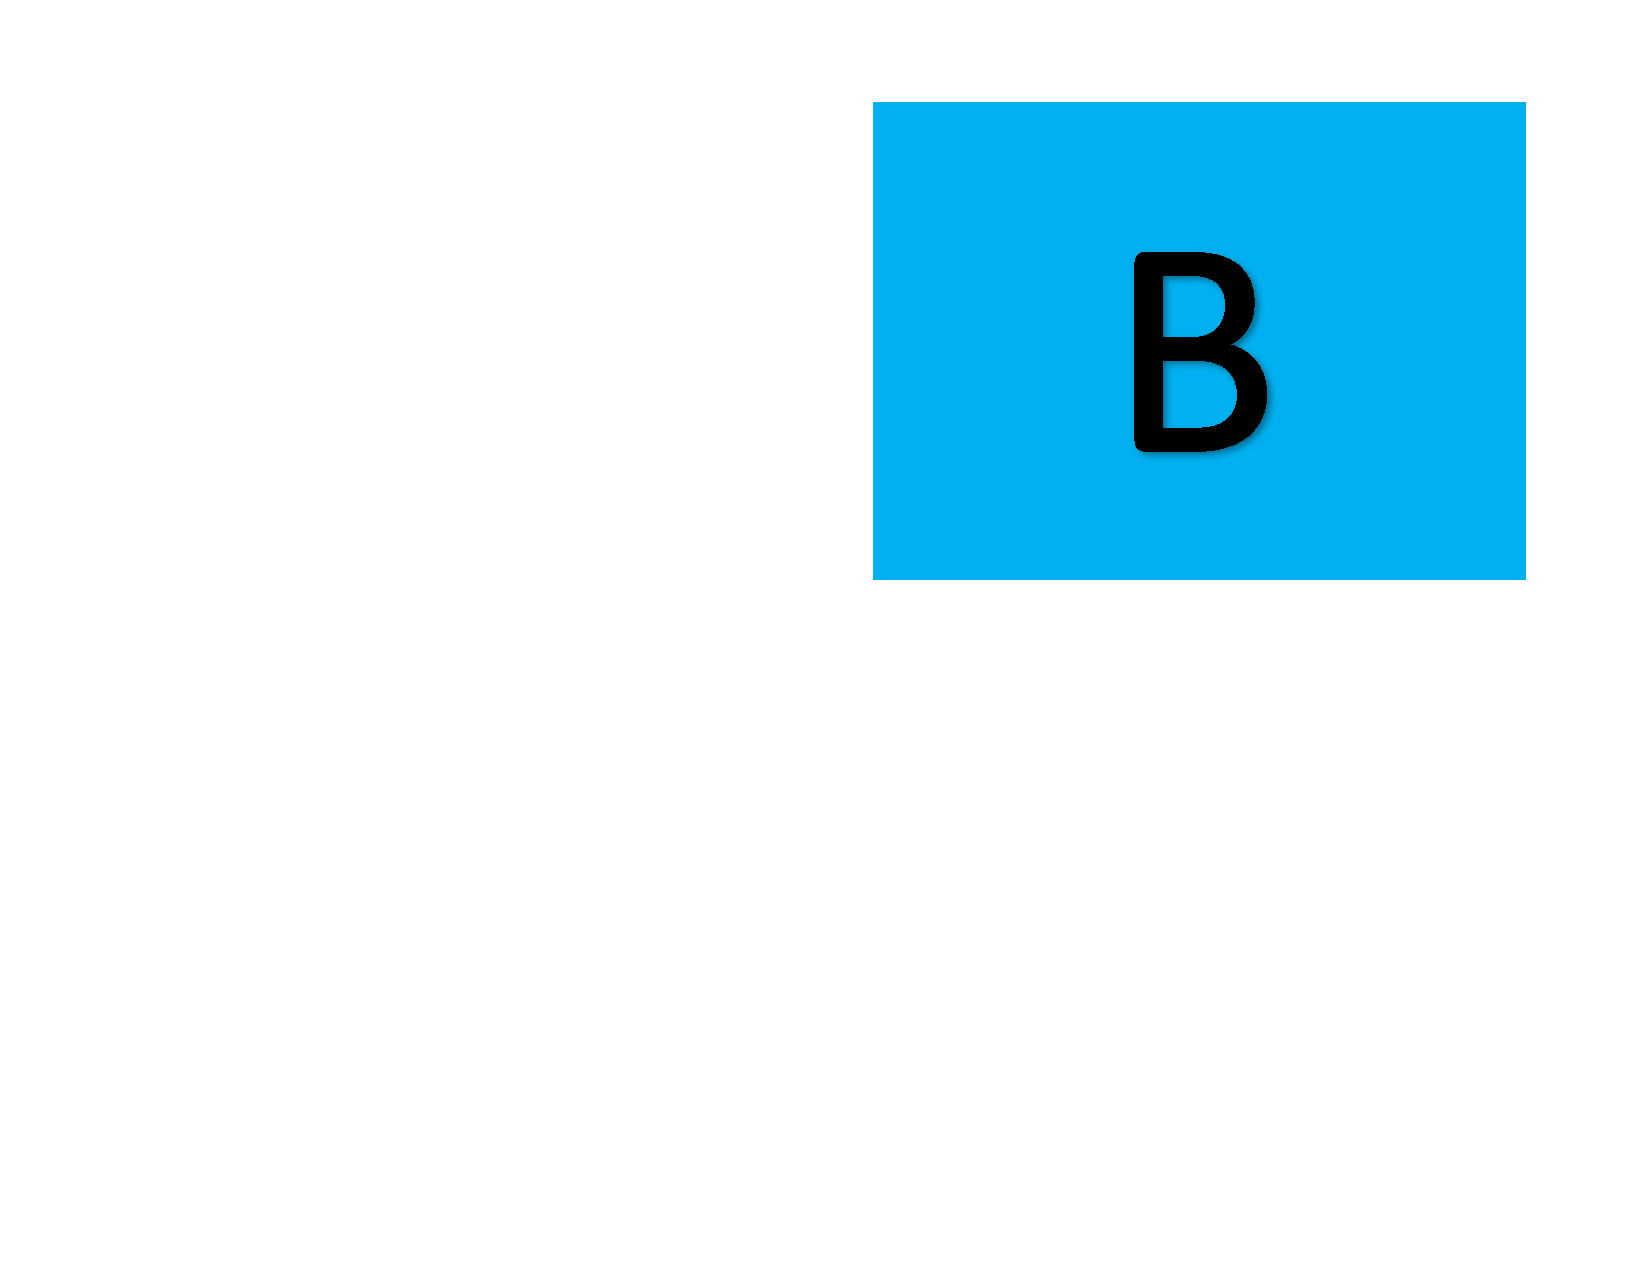
\includegraphics[width=0.8cm,height=0.5cm]{../../Lectures/figures/B}} ]  }
\newcommand*{\citem}{ \item[{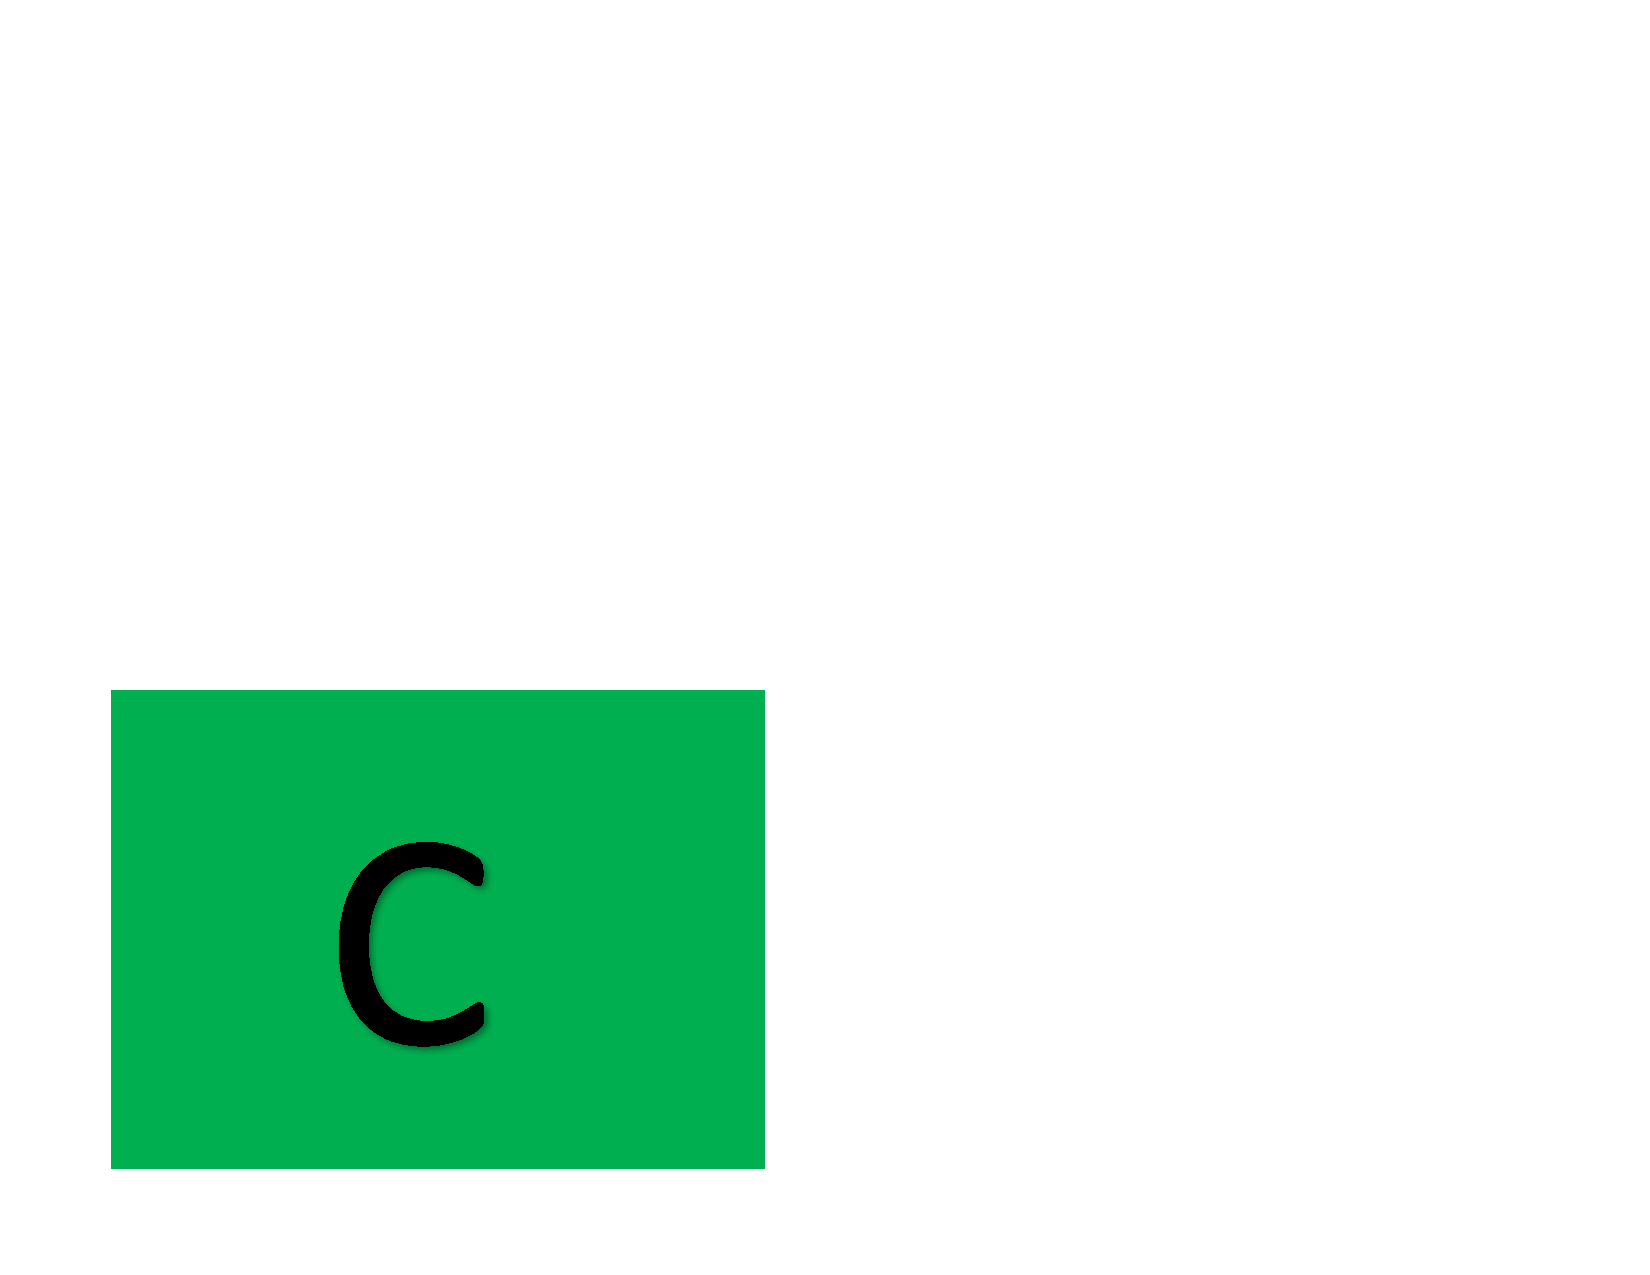
\includegraphics[width=0.8cm,height=0.5cm]{../../Lectures/figures/C}} ]  }
\newcommand*{\ditem}{ \item[{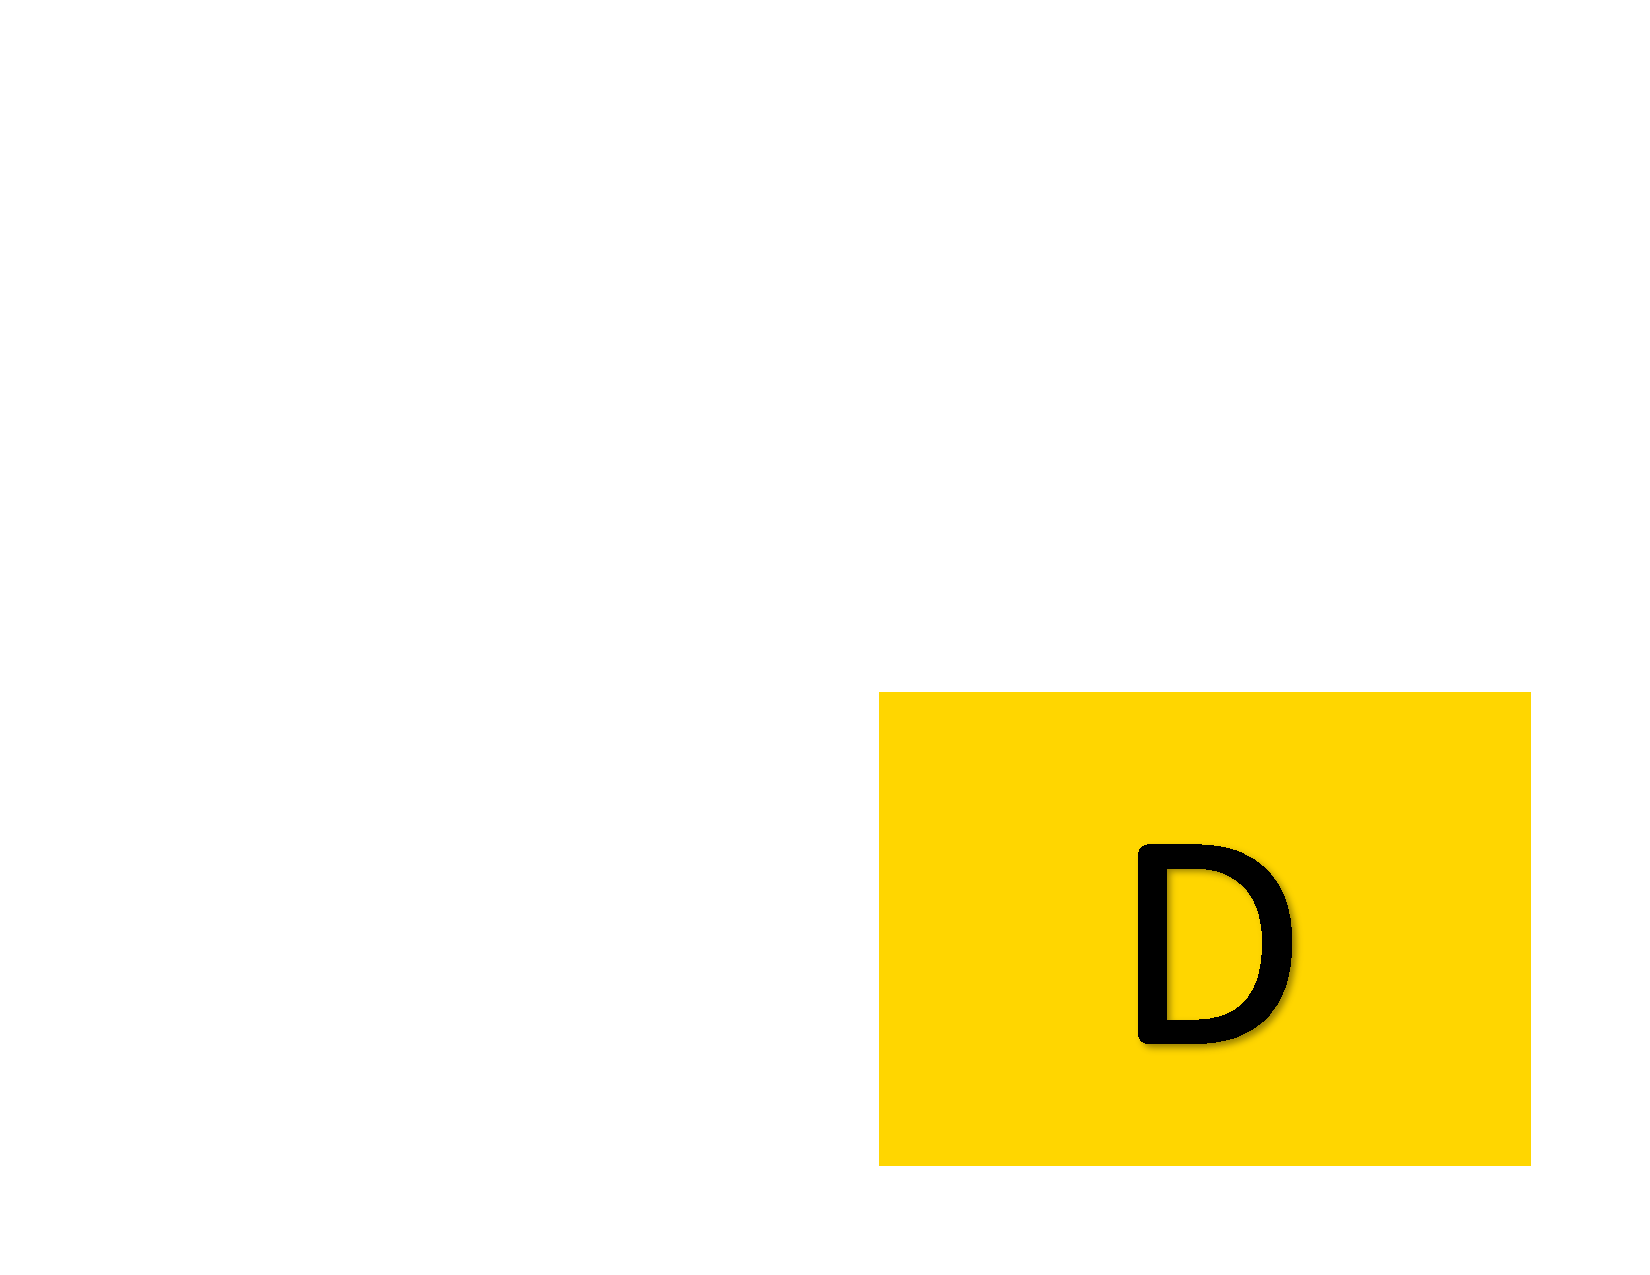
\includegraphics[width=0.8cm,height=0.5cm]{../../Lectures/figures/D}} ]  }
\newcommand*{\eitem}{ \item[{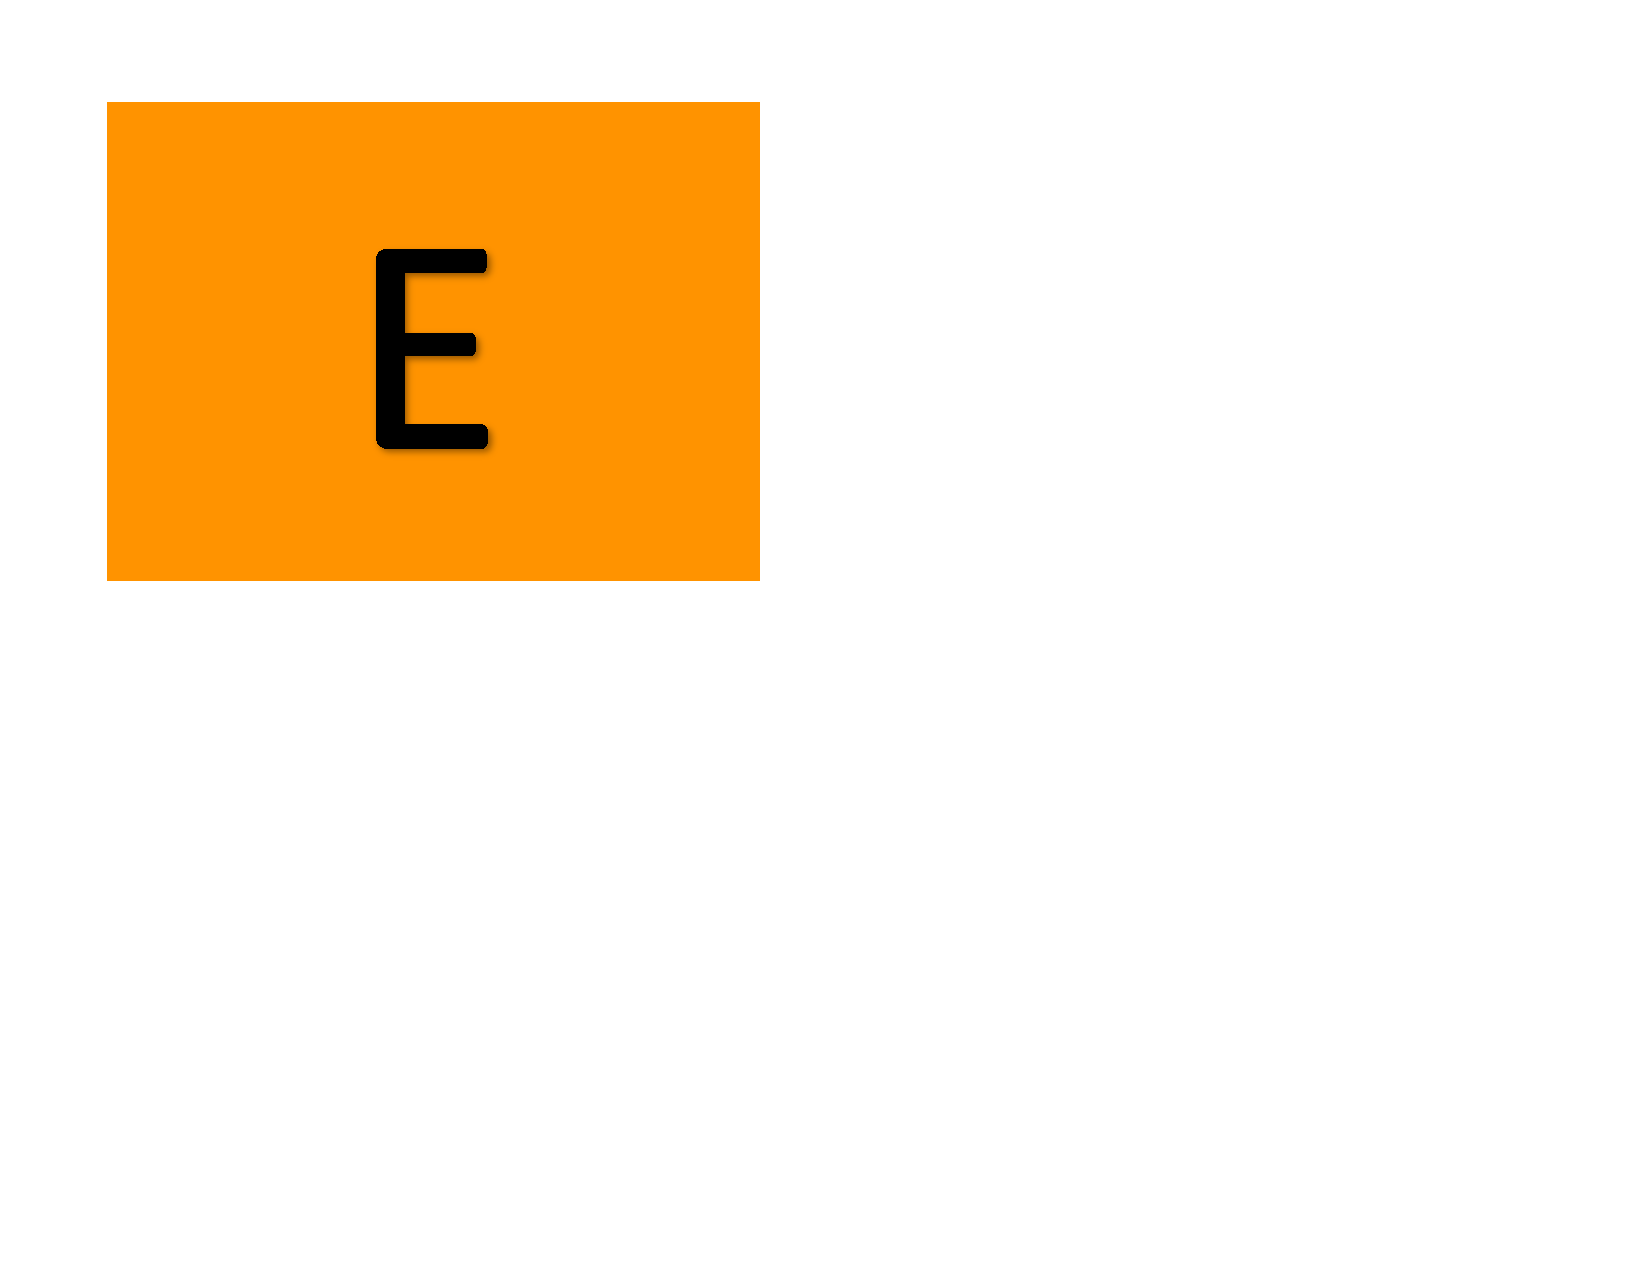
\includegraphics[width=0.8cm,height=0.5cm]{../../Lectures/figures/E}} ]  }
\newcommand*{\fitem}{ \item[{
\includegraphics[width=0.8cm,height=0.5cm]{../../Lectures/figures/F}} ]  }


\newcommand{\hide}[1]{\underline{\phantom{#1 #1}}}

\usepackage{setspace}

\onehalfspacing

\begin{document}
	
	\lecture{13: Finishing DFS; Minimum Spanning Trees}{March 4}
	
	\paragraph{Course Logistics}
	
	\begin{itemize}
		\item Minimum Spanning Tree: Chapter 23
		\item Homework 5 due Friday
	\end{itemize}
	
	\section{The transpose graph and connected component graph}
	If $G = (V,E)$ is a graph, a \emph{strongly connected component} is maximal subgraph $S \subseteq V$ in which every node is reachable from every other node by following paths in $S$. \\
	
	Let $G = (V,E)$ be a graph and assume that $\{C_1, C_2, \hdots , C_k\}$ represent its strongly connected components. 
	
	The \emph{connected component graph} $G^\text{scc} = (V^\text{scc}, E^\text{scc})$ is defined as follows:
	\begin{itemize}
		\item There is a node $v_i \in V^{\text{scc}}$ for each component $C_i$
		\item There is an edge $(v_i, v_j) \in E^{\text{scc}}$ if and only if there is a directed edge between $C_i$ and $C_j$
	\end{itemize}
	\begin{lemma}
		The connected component graph is \hide{ directed acyclic jj}
	\end{lemma}
	
	\vs{5cm}
	
	The \emph{transpose graph} of $G$ is $G^T = (V, E^T)$ where
	\begin{align*}
		E^T = \{ (u,v) \colon (v,u) \in E\}
	\end{align*}
	
	\begin{lemma}
		$G$ and $G^T$ have \hide{the same strongly }
	\end{lemma}
	
	\newpage
	
	
	
	
	
	\section{Strongly Connected Components}
	The following algorithm will compute the strongly connected components of a graph $G = (V,E)$:
	
	\textsc{Strongly-Connected-Components}(G)
	\begin{enumerate}
		\item Find a DFS for $G$ to get finish times $u.F$ for each $u \in V$.
		\item Compute the \emph{transpose graph} $G^T = (V,E^T)$
		\item Find a DFS for $G^T$, but in the main loop of DFS, always visit nodes based on the reverse order of finish times from the DFS of $G$.
		\item Output the vertices of each tree in the DFS of $G^T$. 
	\end{enumerate}
	\newpage
	\paragraph{What is the key to making this work?}
	In the second DFS, we essentially visit all of the nodes in the connected components graph in topologically sorted order.
	
	
\newpage
	\section{Minimum Spanning Trees}
Let $G = (V,E,w)$ be an undirected, connected, weighted graph where $w \colon E \rightarrow \mathbb{R}^+$ maps each edge to a nonnegative weight.


\begin{center}
	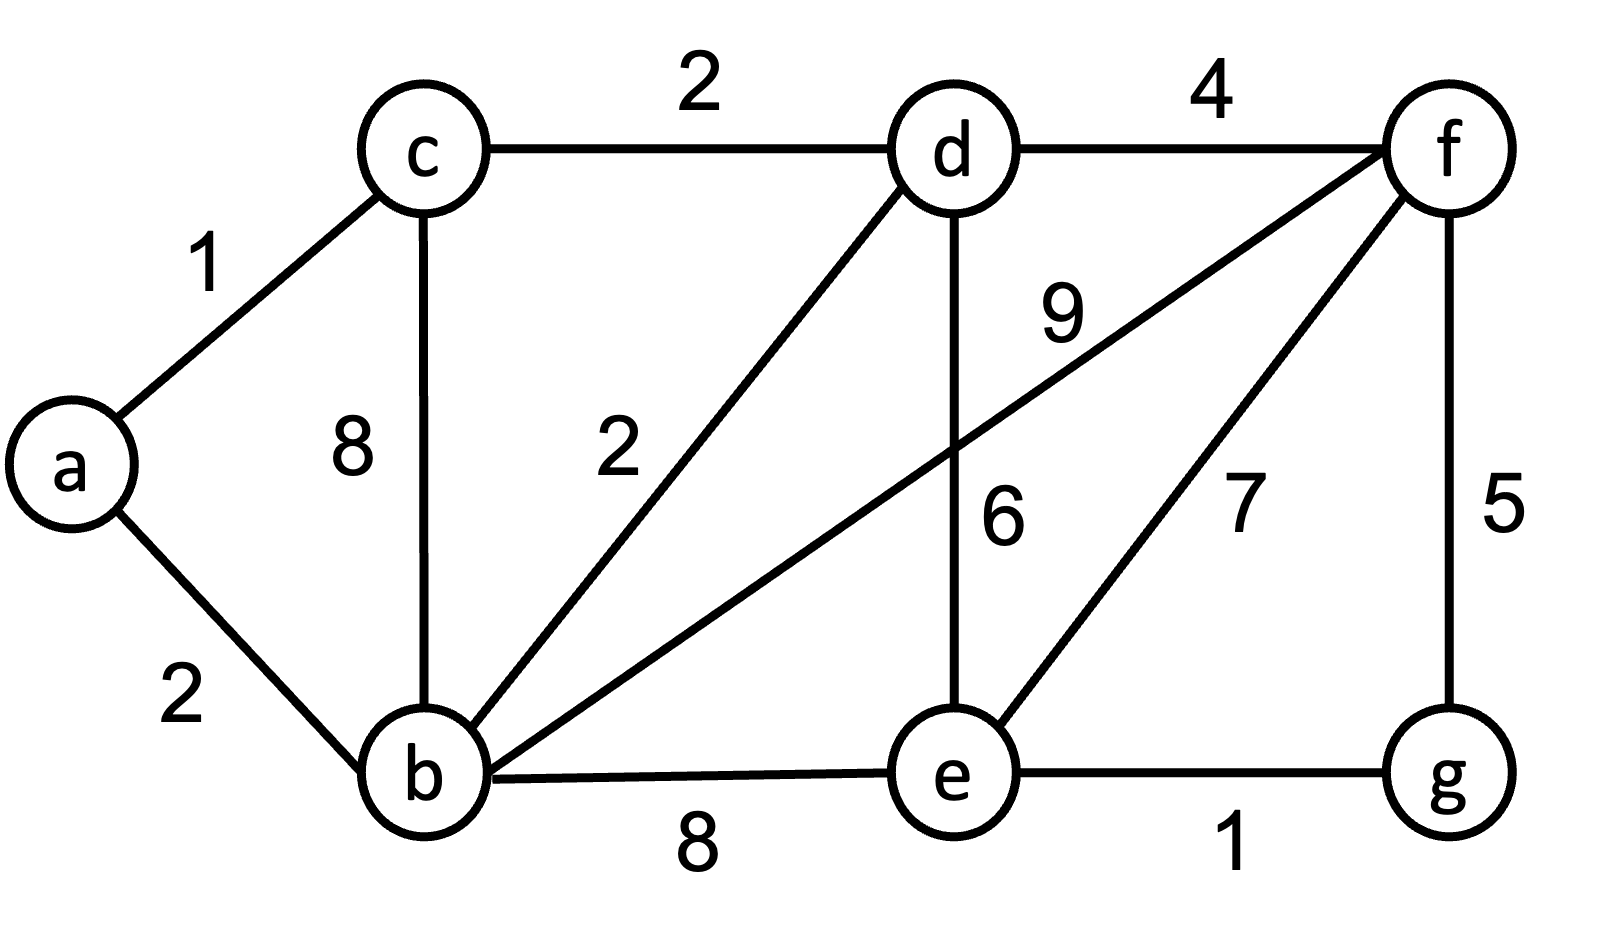
\includegraphics[width = .5\linewidth]{mst-graph.png}
\end{center}

A \emph{spanning tree} of $G$ is a subset of edges $E_T \subseteq E$ such that $T = (V,E_T)$ \hide{is a connect} 

\begin{center}
	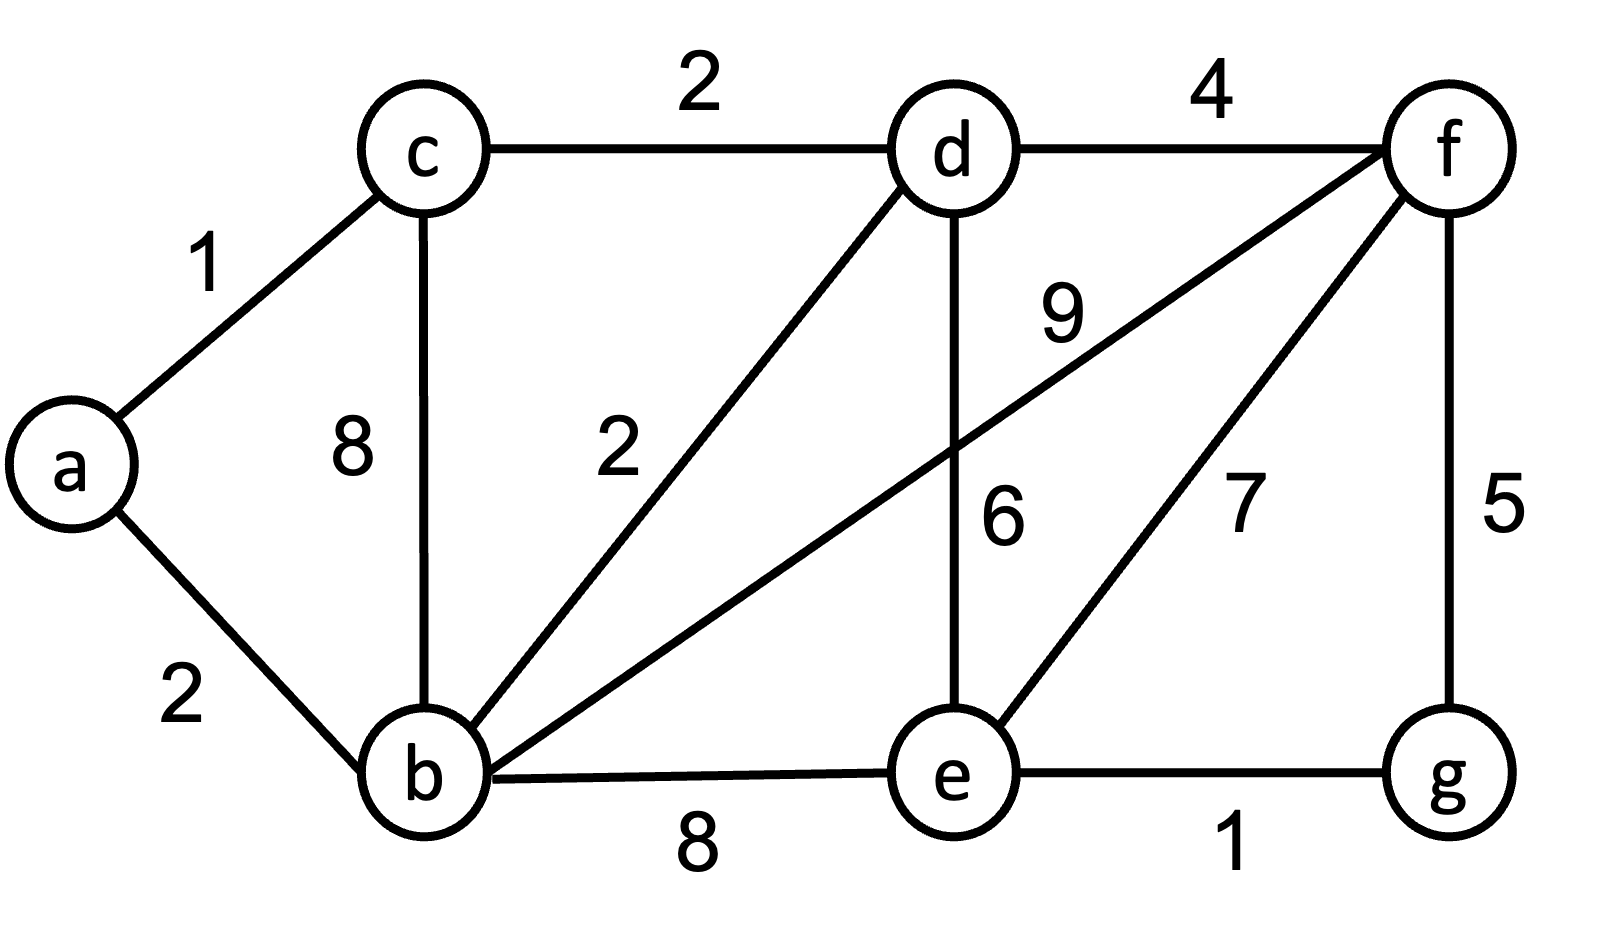
\includegraphics[width = .5\linewidth]{mst-graph.png}
\end{center}

A \emph{minimum spanning tree} of $G$ is a spanning tree $T^*$ that minimizes

\vs{2cm}
over all spanning trees of $G$.

\begin{center}
	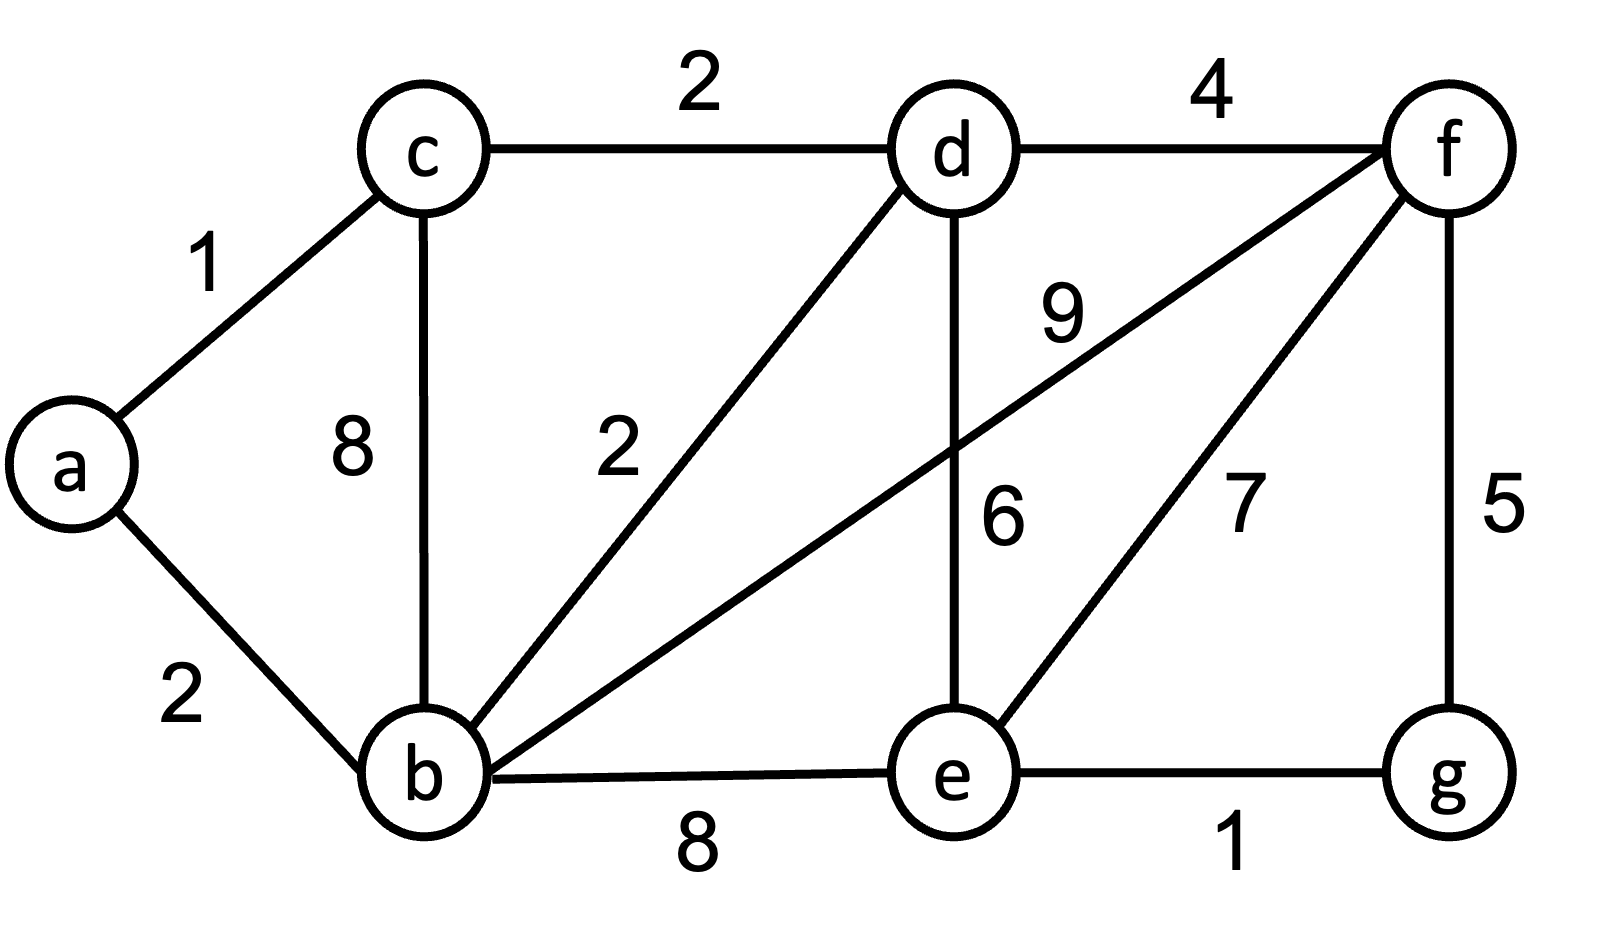
\includegraphics[width = .5\linewidth]{mst-graph.png}
\end{center}

\newpage
\subsection{Minimum Spanning Tree Terminology}
\textbf{Safe Edges.} Let $A$ be a subset of edges that is guaranteed to be in some minimum spanning tree of $G = (V,E)$. An edge $(u,v) \in E$ is \emph{safe} for $A$ if $A\cup \{(u,v)\}$ is contained in some minimum spanning tree of $G$.\\

\textsc{GenericMST}$(G,w)$
\begin{enumerate}
	\item Set $A = \emptyset$
	\item While $A$ is not a spanning tree
	\item \;\;\; find a safe edge $(u,v)$ for $A$
	\item \;\;\; $A \leftarrow A \cup \{(u,v)\}$
\end{enumerate}

The key to implementing this method is \emph{finding a safe edge $(u,v)$ at each step}.\\

\paragraph{Cut terminology}
Let $G = (V,E)$ and $A$ be a set of its edges.
\begin{itemize}
	\item If $S \subseteq V$, we call the partition $(S, V-S)$ a \hide{cut}\\
	\item An edge $(u,v) \in E$ \hide{crosses} the cut $(S, V-S)$ if \hide{one of its endpoint} \\
	\item A cut \hide{respects} $A$ if no edge in $A$ is cut\\
	\item An edge $(u,v)$ is a \hide{light edge} if is has minimum weight among all cut edges. 
\end{itemize}

\newpage
\subsection{Generic greedy strategy}
We define the following \emph{greedy} strategy for choosing a \emph{safe} edge to add to $A$

\textsc{GenericFindSafe}$(G,A,w)$
\begin{enumerate}
	\item Let $(S, V-S)$ be a cut that \emph{respects} $A$
	\item Let $(u,v)$ be a light edge in $(S, V-S)$
	\item Return $(u,v)$
\end{enumerate}
\begin{lemma}
	If $A$ is a subset of the edges in a minimum spanning tree $T$ of $G$, then \textsc{GenericFindSafe} will return a safe edge for $A$
\end{lemma}


\newpage

\subsection{Algorithms of Kruskal and Prim}
Kruskal algorithm and Prim's algorithm are two strategies for creating an MST of $G = (V,E)$.\\

\begin{tabular}{| l | p{7cm} | p{6cm} |}
	\hline
	\textbf{Strategy} & \textbf{What is $A$?} & At each step we add: \\
	\hline
	Kruskal &  \phantom{least weight edge connecting two components} & \phantom{least weight edge connecting two components} \phantom{more of the same stuff right here} \\
	\hline
	Prim & & \phantom{least weight edge connecting tree to another previously unconnected node} \phantom{more of the same stuff right here}\\
	\hline
\end{tabular}

\begin{center}
	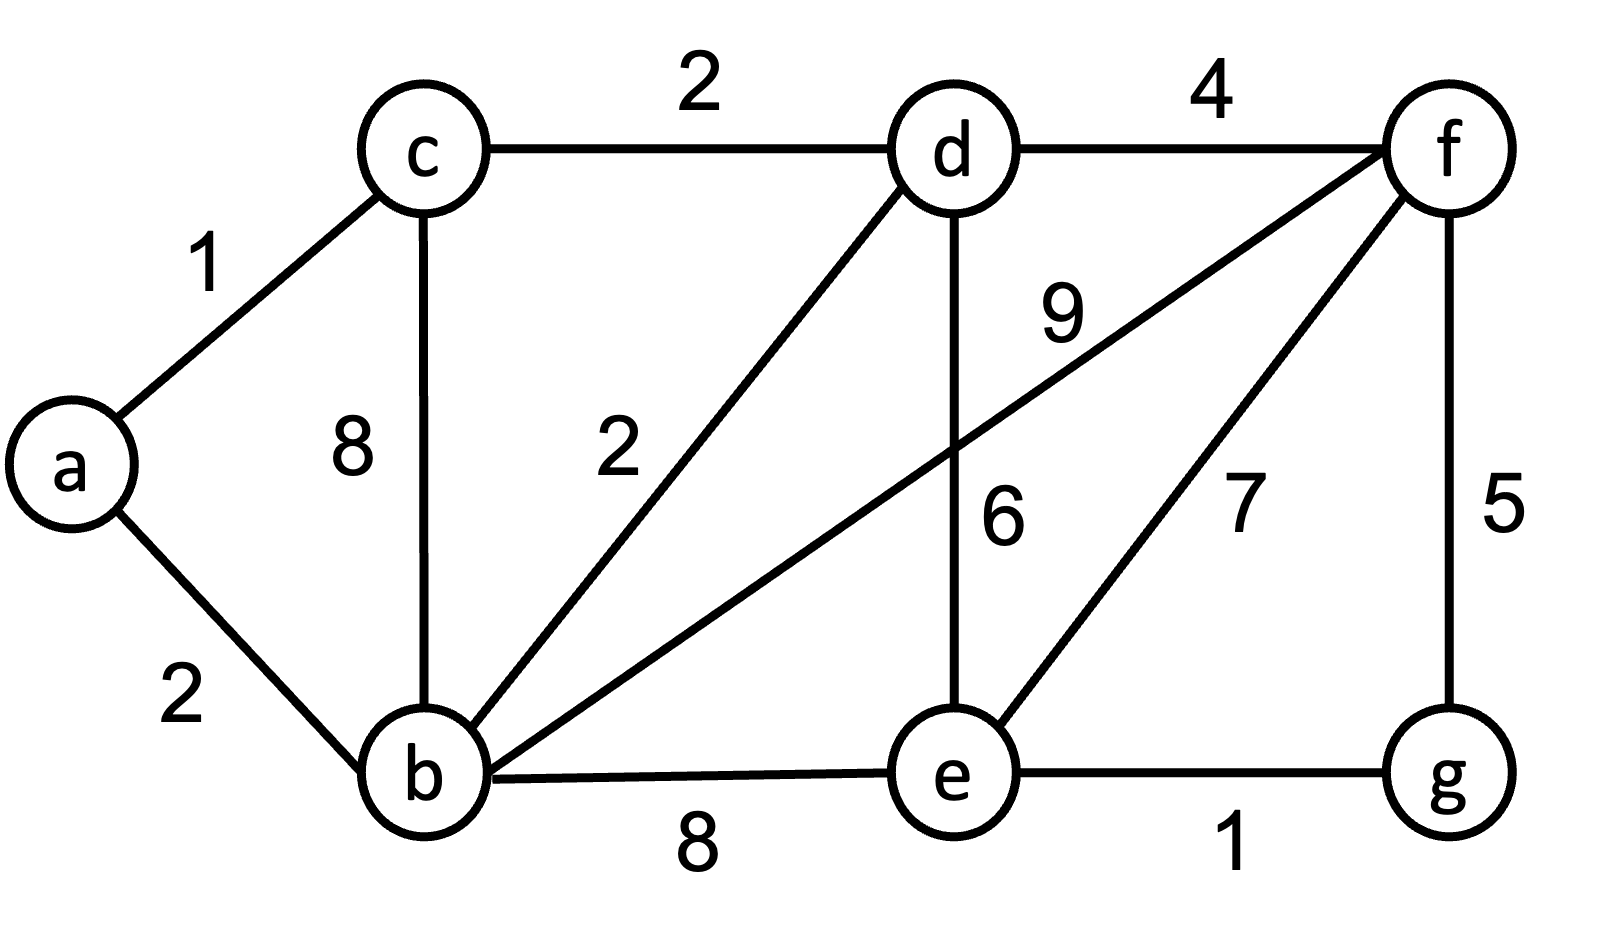
\includegraphics[width = .75\linewidth]{mst-graph.png}
\end{center}

\vs{1cm}

\begin{center}
	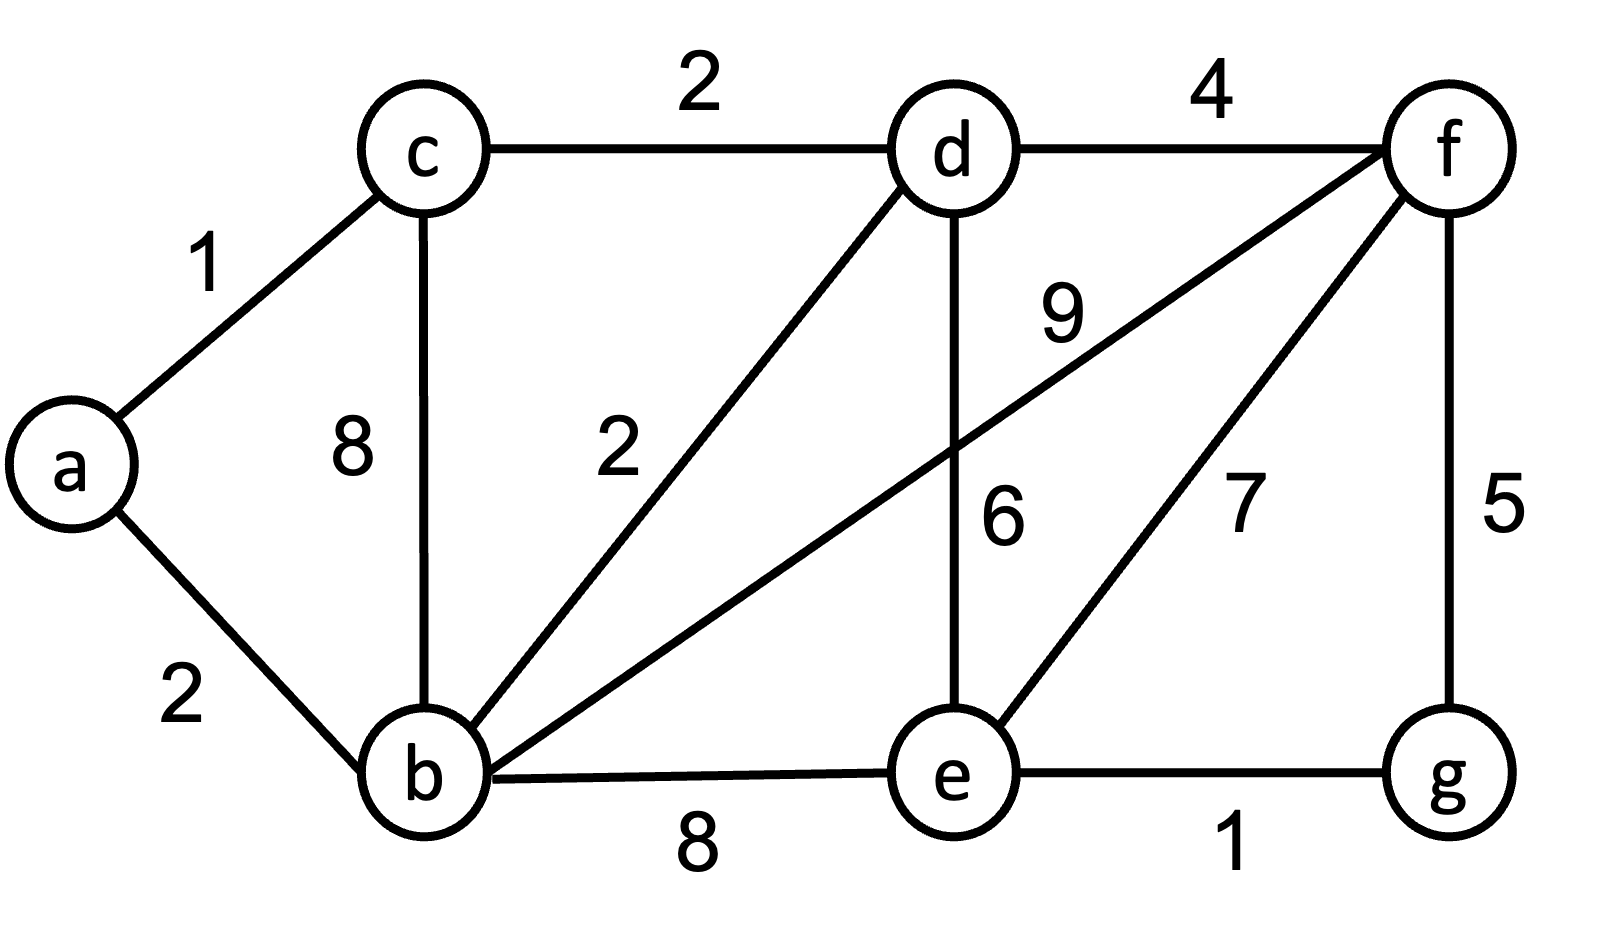
\includegraphics[width = .75\linewidth]{mst-graph.png}
\end{center}

\newpage
\subsection{Prim's Algorithm in More Depth}

During Prim's algorithm, we grow out a tree from an arbitrary starting node $r$. Each node has the following attributes:
\begin{itemize}
	\item $v.\text{parent}$ = parent node of $v$ in the tree we are constructing
	\item $v.\text{key}$ = minimum weight of an edge connecting $v$ to the tree
\end{itemize}
We will use a min-priority queue $Q$ to store the nodes \emph{not in the tree} with their keys, which allows us to find the node with the smallest key in $O(\log V)$ time. 

\begin{algorithm}
	\textsc{MST-Prim}($G,r$)
	\begin{algorithmic}
		\For{$u \in V$}
		\State $u.\text{key} = \infty$
		\State $u.\text{parent} = NIL$
		\EndFor
		\State $r.\text{key} = 0$
		\State $Q = G.V$ 
		\While{$|Q| > 0$}
		\State $u = \textsc{ExtractMin}{Q}$
		\If{$u \neq r$}
		\State Add edge $(u,u.\text{parent})$ to $A$
		\EndIf
		\For{$v \in \text{Adj[u]}$}
		\If{$v \in Q$ and $w(u,v) < v.\text{key}$}
		\State $v.\text{parent} = u$
		\State $v.\text{key} = w(u,v)$
		\EndIf
		\EndFor
		\EndWhile
		\State Return $A$
	\end{algorithmic}
\end{algorithm}

\begin{center}
	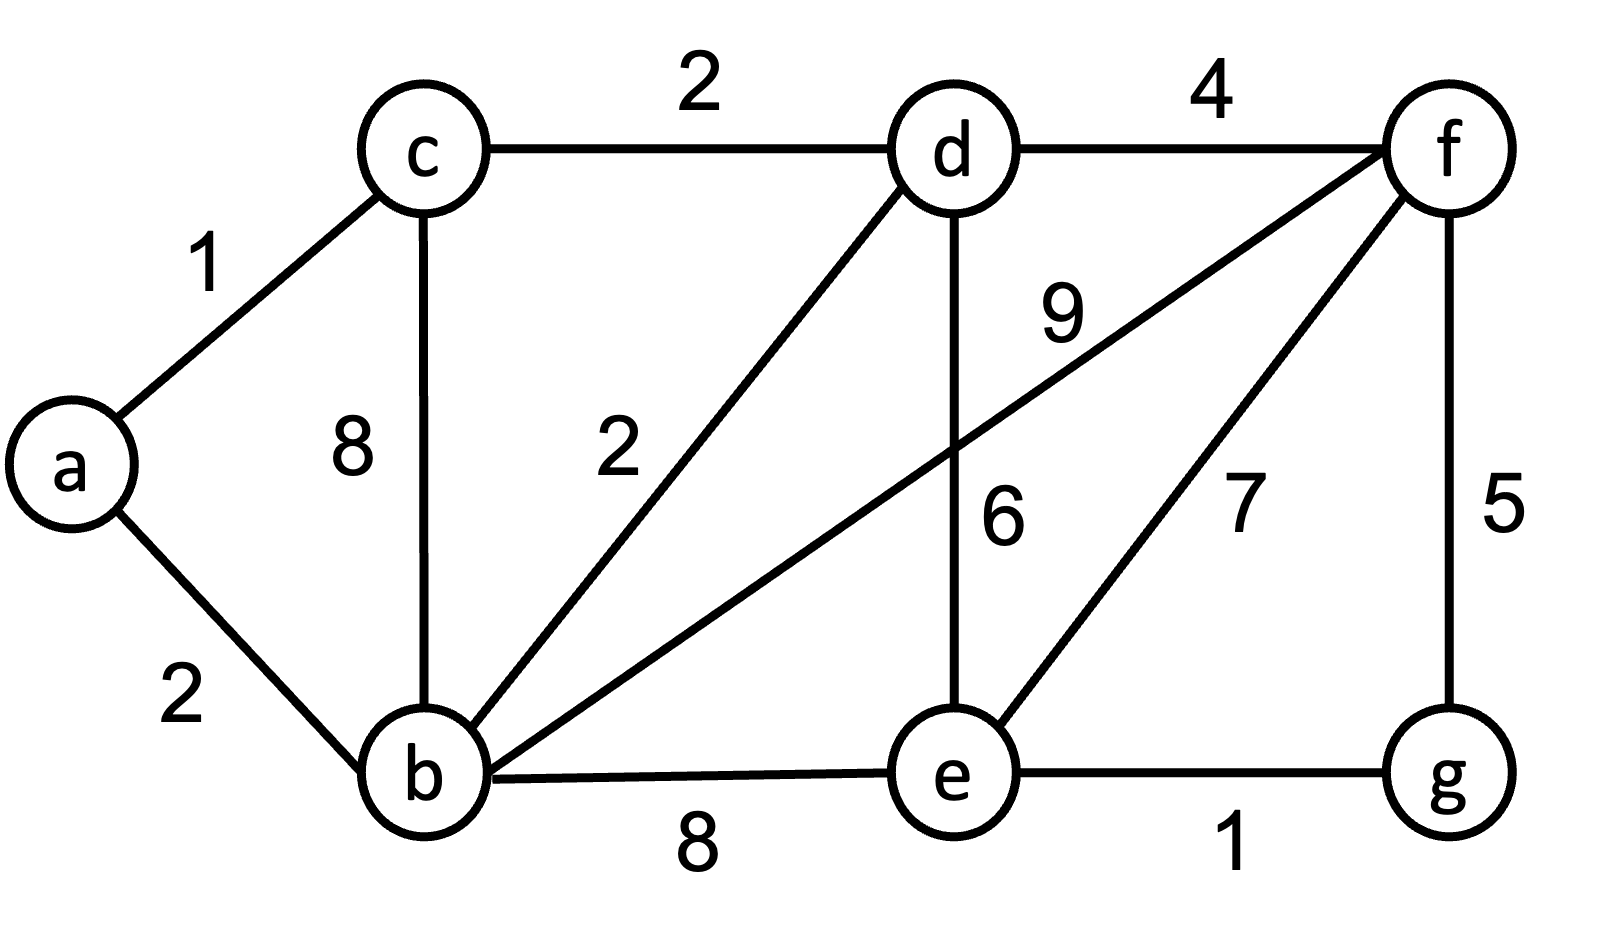
\includegraphics[width = .75\linewidth]{mst-graph.png}
\end{center}

\newpage

\begin{Qu}
	What is the runtime of Prim's algorithm, knowing that it takes $O(\log V)$ time to extract the minimum element from $Q$ or update the key of an element in $Q$?
	\begin{itemize}
		\aitem $\Theta(\log V)$
		\bitem $\Theta(\log E)$
		\citem $\Theta(V \log V)$
		\ditem $\Theta(E \log V)$
		\eitem $\Theta(V^2)$
	\end{itemize}
\end{Qu}

\end{document}
